%\begin{tikzpicture}[>=stealth,scale=0.6,line width=0.8pt]
%\scriptsize
%% % % % % % % % % % % % % % %
% 
%\pgfmathsetmacro{\ticker}{0.125} 
% 
%\coordinate [label=225:0](A) at (0,0);
%\coordinate (B) at (0,5);
%\coordinate (C) at (7.5,5);
%\coordinate (D) at (7.5,0);
%\draw(A)--(B)--(C)--(D)--cycle;
% 
%\coordinate [label=left:{\scriptsize runtime(s)}](E) at ($(B)+(1,0.2)$);
%\coordinate [label=below:{\scriptsize components}](F) at ($(D)+(0,-0.3)$);
% 
%\foreach \i/\texti in {100,300,...,1000} {
%\draw (0.01*\i*0.7,0) --(0.01*\i*0.7,\ticker) node[label=below:\texti]{};
%}
%\foreach \i in {200,400,...,1000} {
%\draw (0.01*\i*0.7,0) --(0.01*\i*0.7,\ticker);
%}
%
%\foreach \j/\textj  in {1,2,3,4} {
%\draw (0,\j) --(\ticker,\j) node[label=left:\textj]{};
%}
%
%
%\coordinate (1) at (1*0.7,0.029);
%\coordinate (2) at (2*0.7,0.079);
%\coordinate (3) at (3*0.7,0.209);
%\coordinate (4) at (4*0.7,0.330);
%\coordinate (5) at (5*0.7,0.729);
%\coordinate (6) at (6*0.7,0.948);
%\coordinate (7) at (7*0.7,1.379);
%\coordinate (8) at (8*0.7,2.102);
%\coordinate (9) at (9*0.7,3.416);
%\coordinate (10) at (10*0.7,4.58);
%\draw(1)--(2)--(3)--(4)--(5)--(6)--(7)--(8)--(9)--(10);
% 
% 
% 
%\end{tikzpicture}
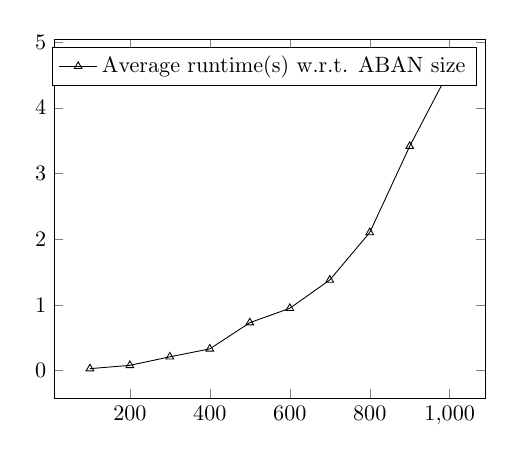
\begin{tikzpicture}[scale=0.8]
    \begin{axis}%[legend pos=north west]
       \addplot[mark=triangle] coordinates{
        (100,0.029)
        (200,0.079)
        (300,0.209)
        (400,0.330)
        (500,0.729)
        (600,0.948)
        (700,1.379)
        (800,2.102)
        (900,3.416)
        (1000,4.58)
        };
        \addlegendentry{Average runtime(s) w.r.t. ABAN size}
    \end{axis}
\end{tikzpicture}